\section{Measurements}
\label{sec:measurements}

\subsection{Preparations and calibration of the setup}
\label{sub:preparations_and_calibration_of_the_setup}
\subsubsection{Controlling the setup with the oscilloscope}
\label{ssub:Controlling the setup with the oscilloscope}
See Table~\ref{tab:config} for the first configuration. 
First we measured the signal from the detector and Photomultiplier. We noticed
that the peaks of shape were at irregular points in time. We exchanged the left for the right side
of the photomultiplier, but did not observe a crucial dependence. Also rotating the sample did not
change the result significantly. Now we removed the oscilloscope and appended the Multichannelanalyzer,
in order to measure the energy spectrum. \\
\\
 \begin{minipage}{\textwidth}
  \begin{minipage}[b]{0.49\textwidth}
    \centering
    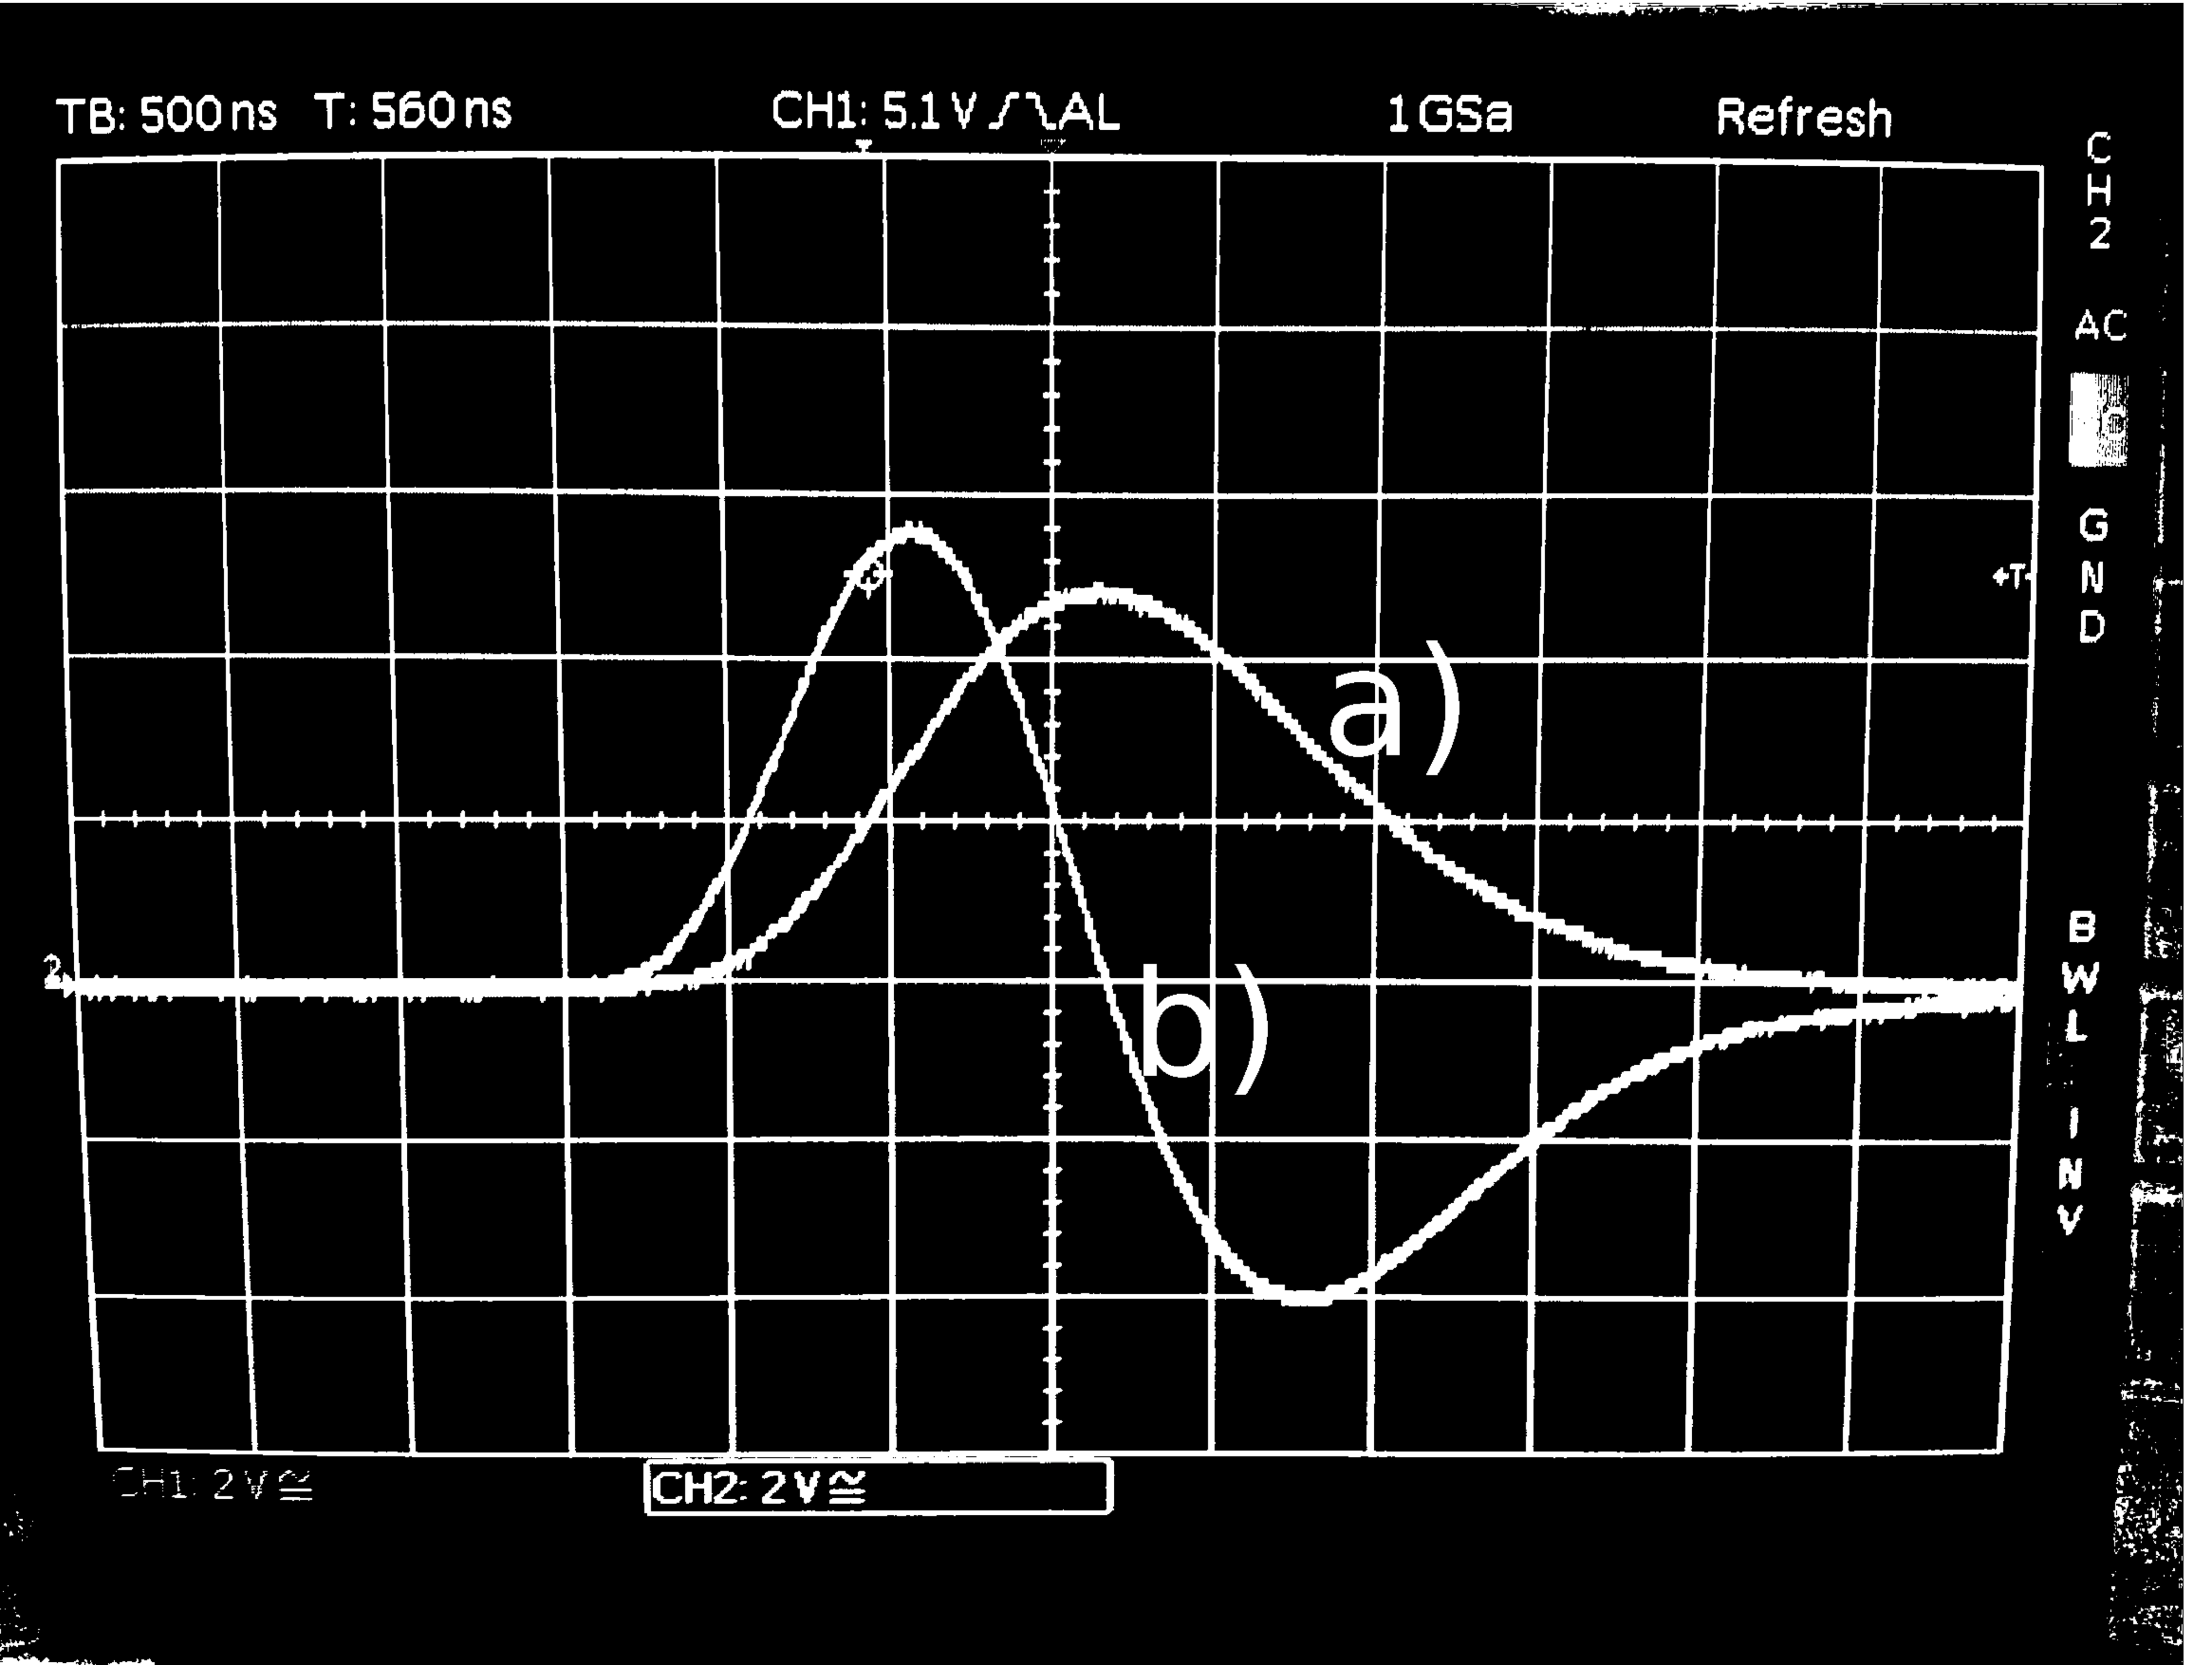
\includegraphics[width=0.8\linewidth]{figures/uni_bipolar2}
    \captionof{figure}{Oscillscope: a) refers to the unipolar channel and b) to 
the bipolar channel.}
  \end{minipage}
  \hfill
  \begin{minipage}[b]{0.49\textwidth}
    \centering
 \begin{tabular}{|l|l|}
     \hline
    course grain & 100\\
    gain    &   10.0 \\
    sharpening time &   0.5 \\
    sample & position 1\\
    PM & Right Side\\
    output & unipolar MCA\\
           & bipolar delay\\
     BLR & AFJ \\
     +/- & Pos \\
     delay & out\\
     \hline
\end{tabular}
\label{tab:config}
  \captionof{table}{Configuration of MA, MCA in measurement 2.1.1.}
    \end{minipage}
\end{minipage}

\subsubsection{Measuring the full energy spectrum}
\label{ssub:Measuring the full energy spectrum}
We increased the gain to 8.6 and the coarse gain to 200 of the MA, such that a observed spectrum 
was distributed of the entire range of bins, in order to be able to decide which detector and position would
be suitable. See Table~\ref{tab:config2} for our configuration of the setup. See
Figure~\ref{fig:measure2.1} for the figures of the measurement 2.1.
\begin{table}[htp]
    \begin{tabular}{|l|l|l||l|l|l|}
        \hline
        2.1a) & Positions:  & Pos1         & 2.1b) & Positions:  & Pos1\\
              & PM          & right        &       & PM          & left \\
              & Time        & $360\pm1$sec &       & Time        & $380\pm1$sec \\
        \hline 
        2.1c) & Positions:  & Pos2         & 2.1d) & Positions:  & Pos2         \\
              & PM          & right        &       & PM          & left \\
              & Time        & $402\pm1$sec &       & Time        & $368\pm1$sec \\
        \hline 
        2.1e) & Positions:  & Pos2         \\
              & PM          & left \\
              & Time        & $360\pm1$sec \\
    \cline{1-3}
    \end{tabular}
  \caption{Configuration in measurement 2.1 of Position, PM and integration time.}
    \label{tab:config2}
\end{table}

\begin{figure}
    \begin{subfigure}[b]{\picwidth}
        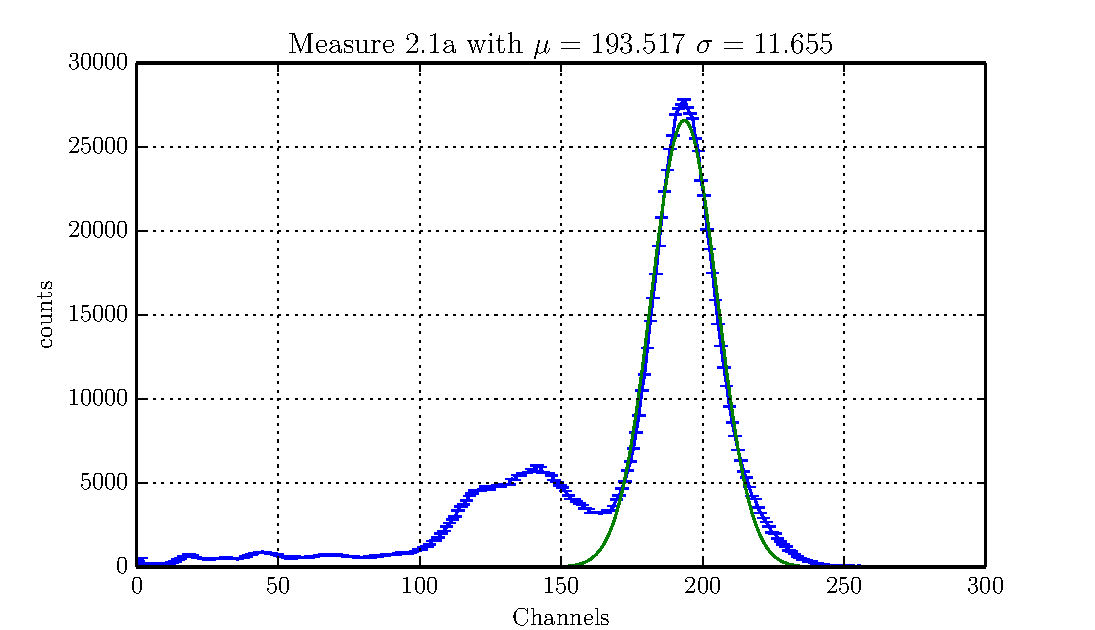
\includegraphics[width=\textwidth]{analysis/figures/plot2_1a}
        \caption{}
    \end{subfigure}\qquad
    \begin{subfigure}[b]{\picwidth}
        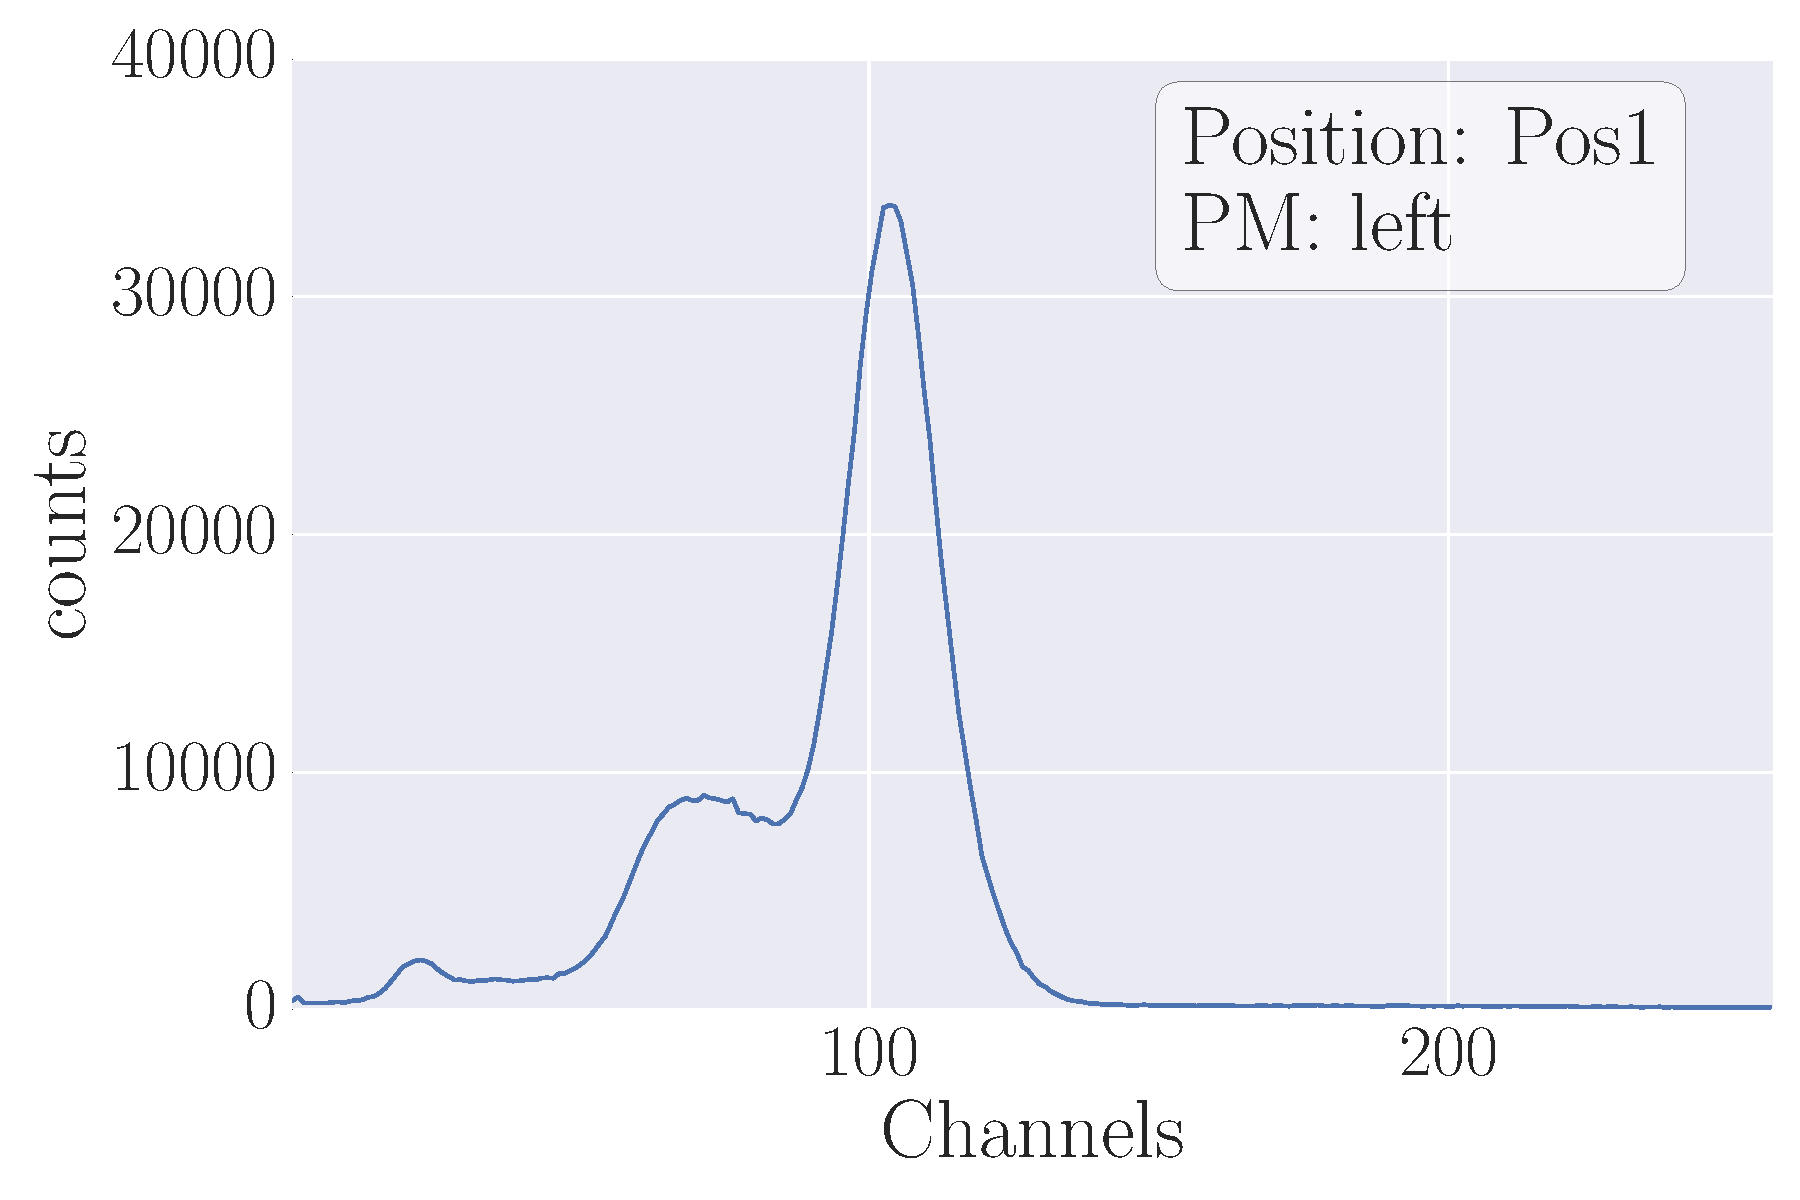
\includegraphics[width=\textwidth]{analysis/figures/plot2_1b}
        \caption{}
    \end{subfigure}
    \begin{subfigure}[b]{\picwidth}
        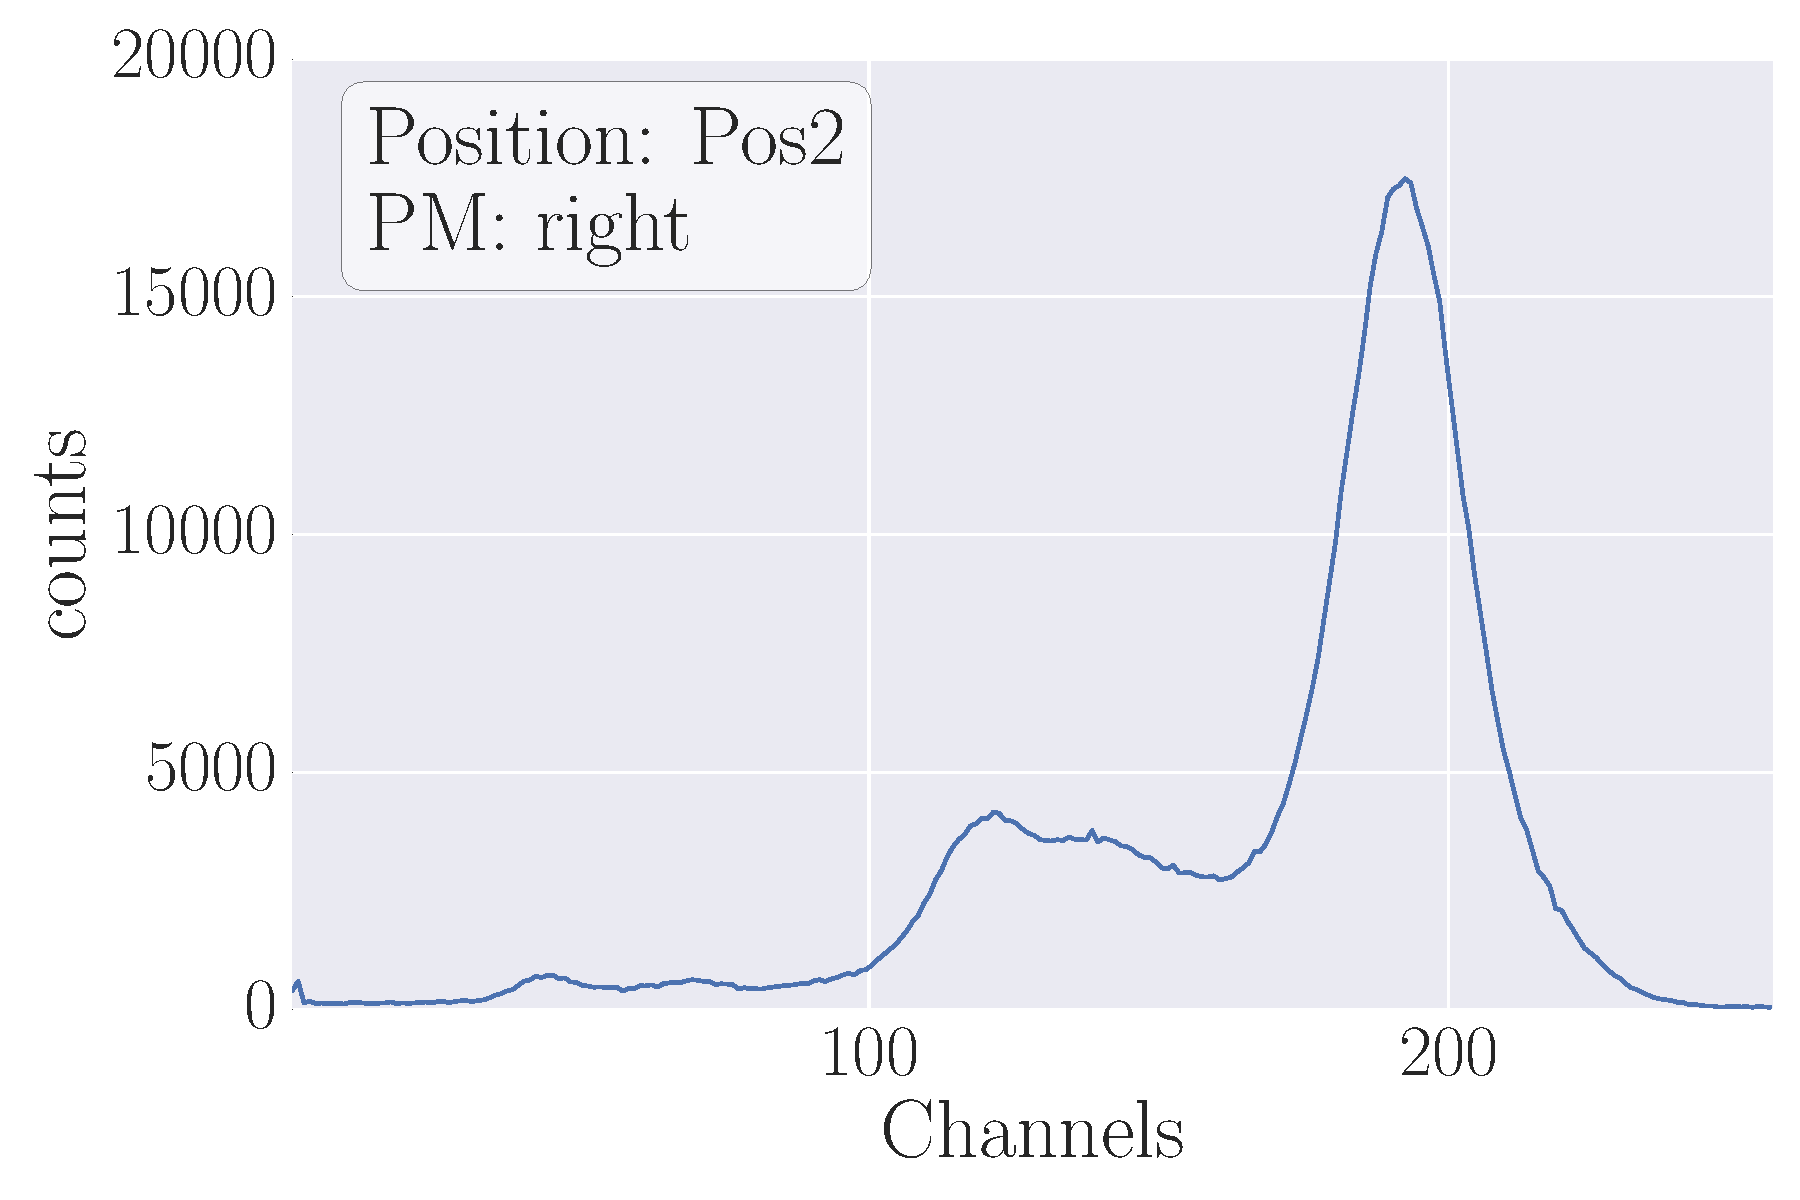
\includegraphics[width=\textwidth]{analysis/figures/plot2_1c}
        \caption{}
    \end{subfigure}
    \begin{subfigure}[b]{\picwidth}
        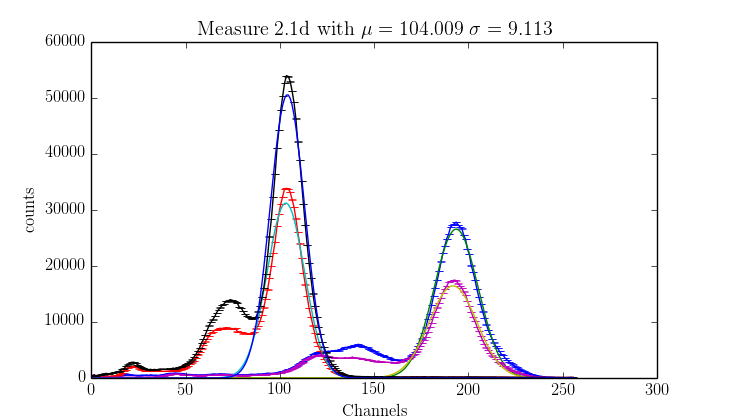
\includegraphics[width=\textwidth]{analysis/figures/plot2_1d}
        \caption{}
    \end{subfigure}
    \begin{subfigure}[b]{\picwidth}
        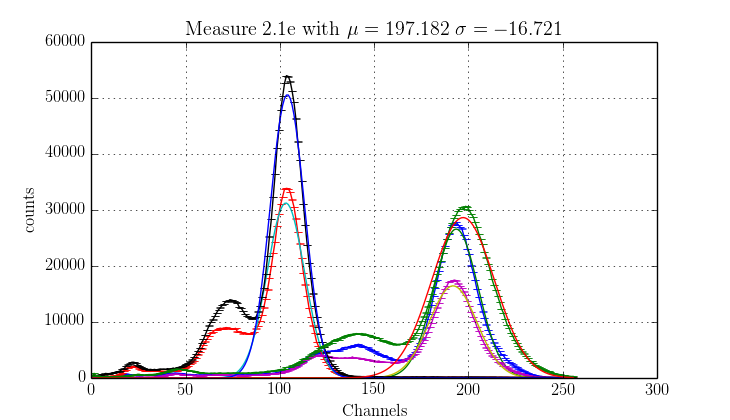
\includegraphics[width=\textwidth]{analysis/figures/plot2_1e}
        \caption{}
    \end{subfigure}
    \caption{Energy spectra with respect to the channels of the MCA, which we prescribed by
        measurements 2.1 (a) - (e).}
    \label{fig:measure2.1}
\end{figure}
\clearpage
\subsection{Measuring delayed coincidences}
\label{sub:measuring_delayed_coincidences}
\subsubsection{Setting the energy window}
\label{ssub:Setting the energy window}
From the results of the last chapter we have decided to chose position 1, which refers to measurements 2.1 a)
and 2.1 b). We only show the configuration of the successfull run with the right energy window chosen.
For the other configurations please see the appended records. For the the time delay we chose
$\Delta t = 140$ns.\\\\ 
 \begin{minipage}{\textwidth}
  \begin{minipage}[b]{0.49\textwidth}
   \begin{tabular}{|l|l|}
        \hline
       14.4 keV signal & right detector \\
       122 keV signal & left detector \\
       coarse gain & 200 \\
       gain & 8.6 \\
       Shaping time & $0.5\mu$s \\
        \hline
   \end{tabular}

  \captionof{table}{Configuration of MA1}
  \end{minipage}
  \hfill
  \begin{minipage}[b]{0.49\textwidth}
    \centering
   \begin{tabular}{|l|l|}
        \hline
       Lower Level & $4.75\pm0.05$ \\
       Upper Level & $3.72\pm0.05$ \\
       Delay & 1.0 (minimum possible) \\
        walk ADJ & $0.1 - 1.1\mu$s (NOR)  \\
       Pos Out & Linear Gate ``enable''\\
        \hline
   \end{tabular}
  \captionof{table}{Configuration of SCA1}
\end{minipage}
\end{minipage}
\begin{minipage}{\textwidth}
  \begin{minipage}[b]{0.49\textwidth}
   \begin{tabular}{|l|l|}
        \hline
       coarse gain & 500 \\
       gain & 8.6 \\
       Shaping time & $0.5\mu$s \\
       input & right detector \\ 
        delay & out \\
        \hline
   \end{tabular}

  \captionof{table}{Configuration of MA2}
  \end{minipage}
  \hfill
  \begin{minipage}[b]{0.49\textwidth}
    \centering
   \begin{tabular}{|l|l|}
        \hline
       Lower Level & $2.02\pm0.05$ \\
       Upper Level & $3.04\pm0.05$ \\
       Delay & 1.0 (minimum possible) \\
        walk ADJ & $0.1 - 1.1\mu$s (NOR)  \\
       Pos Out & Linear Gate ``enable''\\
        \hline
   \end{tabular}
  \captionof{table}{Configuration of SCA2}
\end{minipage}
\end{minipage}
\clearpage
\subsubsection{Conduction of the experiment over night}
The measurement ran about 14 hours over night. See Figure~\ref{fig:4_1} for the visualization.
\label{ssub:Conduction of the experiment over night}

\begin{figure}[htpb]
    \centering
    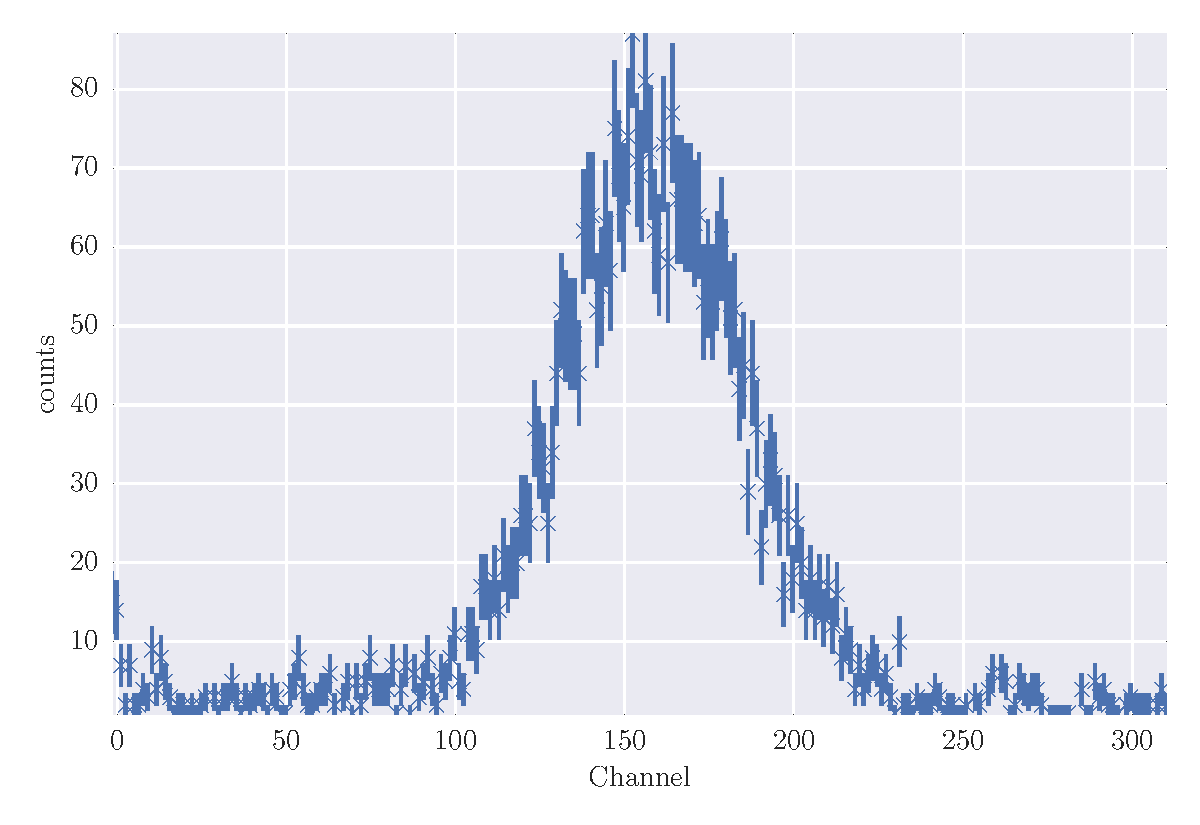
\includegraphics[width=1.0\linewidth]{analysis/figures/plot4_1}
    \caption{Measurement 4.1: $\Delta t $}
    \label{fig:4_1}
\end{figure}

\begin{figure}[htpb]
    \centering
    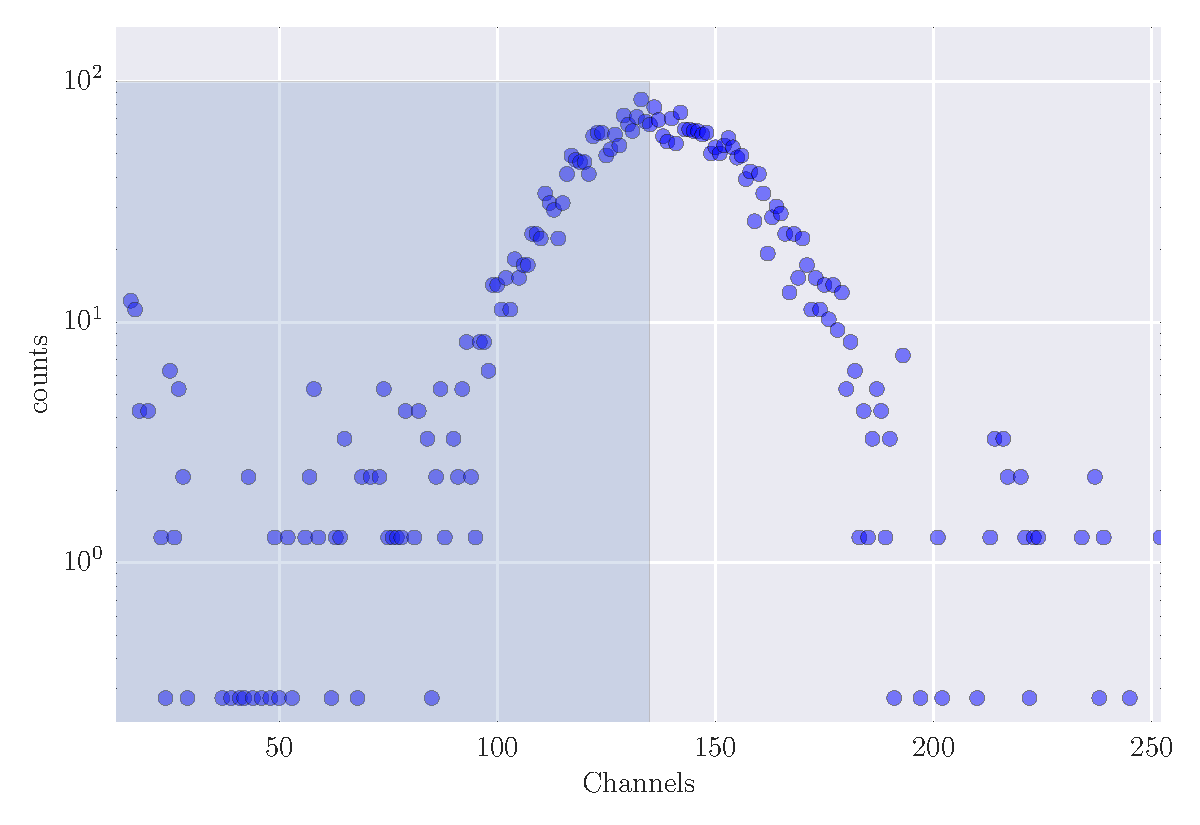
\includegraphics[width=1.0\linewidth]{analysis/figures/plot4_1_log}
    \caption{Measurement 4.1: $\Delta t $}
    \label{fig:4_1log}
\end{figure}


\begin{figure}[htpb]
    \centering
    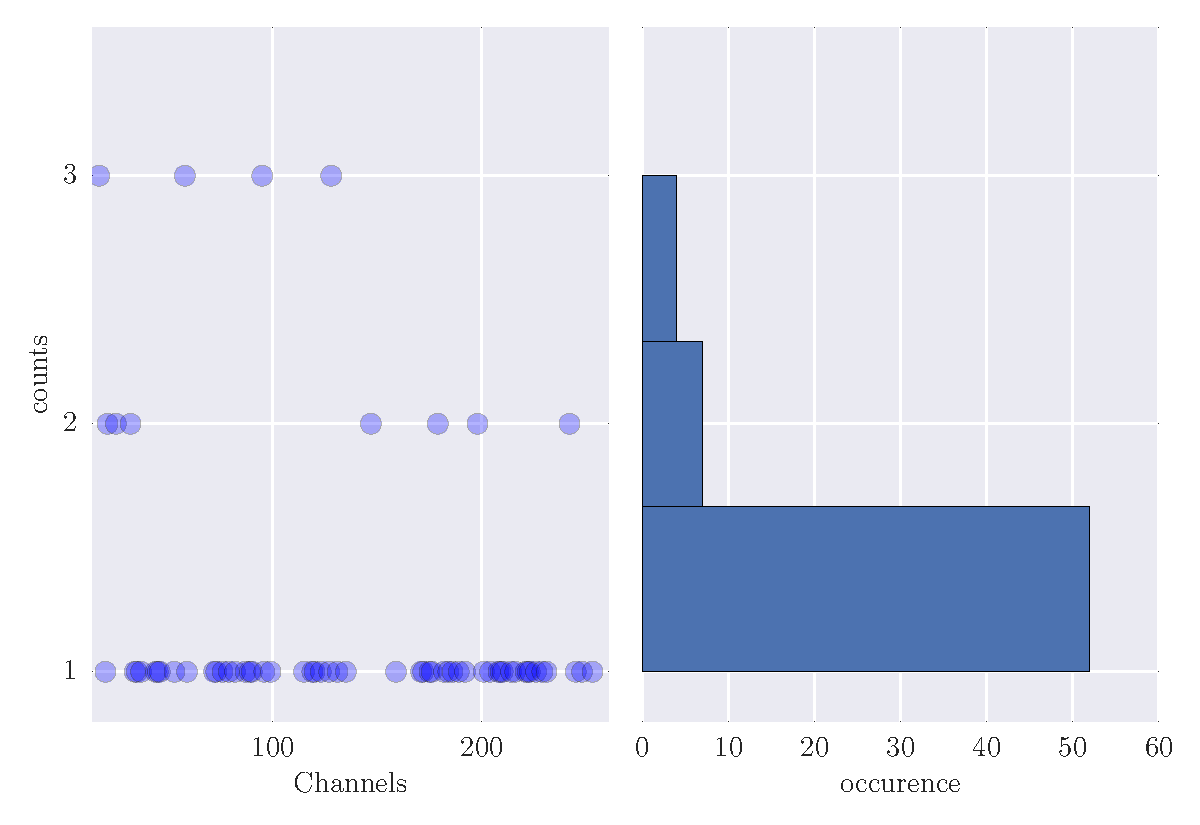
\includegraphics[width=1.0\linewidth]{analysis/figures/plot5_1_hist}
    \caption{Measurement 5.1: Random coincidences and their histogram.}
    \label{fig:5_1}
\end{figure}

